\documentclass{article}
\usepackage{apacite}
\usepackage[english]{babel}
\usepackage[utf8x]{inputenc}
\usepackage{amsmath}
\usepackage{basic} % refers to the style we're using, basic.sty
\usepackage[colorinlistoftodos]{todonotes}

\begin{document}

\title{Contrasting the Branding Effect of Cost Per View vs Cost Per Click Campaigns}
\author{Chad Crowe}

\maketitle

\begin{abstract}
%Alt: When internet users interact with a page, they see both images and text. When predicting how  users will interact with content, traditional algorithms are limited to a single modality--either text or images. We propose a novel algorithm that allows a combination of both text and image features to be used to train a machine learning model to predict user interactions based on page content.  This research demonstrates...

Existing works have predicted user behavior on social media using either image or text data. This research takes a further step with a methodology and implementation that combines image and text data to predict user behavior on social media.  The combined model outperforms text-only or image-only models for predicting user comment sentiment, and user actions for sharing, liking, and commenting on content for 350k Facebook user generated content (UGC) posts. The result is a validated methodology for modeling user behavior on social media.

\end{abstract}
  
\section{Introduction}

\subsection{Machine Learning on Social Media Data}

Existing research recognizes the value of modeling user behavior on social media using machine learning models \cite{Li2015, 8029313, Ohsawa2013, Liu2012, Li2015}. This pattern of research reflects the desire to understand consumer behavior on social media \cite{Fisher2009}. The studies have focused on particular metrics, including user click-through rates \cite{Li2015}, user interaction with Facebook posts \cite{8029313}, predicting user tendency to follow pages \cite{Ohsawa2013}, and user sentiment \cite{Liu2012,Wang2015}. A large amount of research is concerned with better understanding user behavior on social media.

The existing research understands user behaviors through behavior models, which often include machine learning models \cite{Li2015, 8029313, Ohsawa2013, Liu2012, Li2015}, such as through statistical models \cite{Li2015}, neural networks \cite{8029313}, text idf models \cite{Ohsawa2013}, opinion mining \cite{Liu2012}, and sentiment analysis of images \cite{Wang2015}. This research demonstrates the usefulness of user behavior models for gaining insight into understanding user social media behavior. Further research can build upon this methodology of creating and validating user behavior models to better understand user behavior.

Convolutional Neural Networks (CNNs) are often used for modeling social media data with images.  They have been used for gender classification \cite{Hassner2015}, for visual sentiment \cite{Segalin2017, Xu2014}, to detect sarcasm on Twitter \cite{Poria2016}, for detecting stress in social media images \cite{Lin2014}, to perform social media profiling \cite{Segalin2017}, to predict social media popularity \cite{Gelli2015}, and to predict which posts will receive the post clicks \cite{Khosla2014}. CNNs are the standard in the realm of social media for image analysis \cite{Hassner2015}. 

\subsection{Gap}

However, a gap exists in current research, primarily the use of single-data types to model user behavior toward media comprised of multiple data types. Studies predict user interaction with posts based on text and time data \cite{8029313}, however, posts are comprised of image data too. A similar approach is taken for predicting whether a user will follow a Facebook page via NLP techniques \cite{Ohsawa2013}, but which fail to account for the effect of images.  Both using text sentiment or opinion mining \cite{Liu2012} to understand user sentiment fail to capture that users make use of image and texts. Existing models of user behavior tend to rely only on text data.

The situation is made worse when evaluating image-based studies, which fail to incorporate text data into their modeling of user behavior. An example is doing a sentiment analysis of posts with images \cite{Wang2015} but failing to incorporate post data in the model. Each of the cited CNN models also failed to incorporate text-data for predicting gender classification, detecting sarcasm, profiling, and for predicting social media popularity \cite{Hassner2015, Poria2016, Segalin2017, Gelli2015}. Existing image-based models fail to incorporate text data in their analysis.

\subsection{Significance of Methodological Application for Industry}

The application of this study's method is modeling user interaction with FGC social media posts. FGC posts are cultivated by advertisers for the purpose of influencing user behavior. Given the applied aspect of this research, it is worth outlining its applied significance. The study applies to brands on social media who seek to influence users with their posts.

Advertisers are most concerned with social media metrics, especially those that promote engagement \cite{Tiago2014}, which include click-through rate (CTR), brand awareness, and word-of-mouth buzz. Advertisers associate theses with advertisement return on investment (ROI), which is known as the Holy Grail of social media \cite{Fisher2009}. However advertiser calculate ROI, it often includes an increase in user interaction \cite{Romero2011, Schacht2015}. This study successfully models user engagement, which is of great interest advertisers and social media platforms.  

%Our text and image architecture for predicting advertisement performance utilizes deep learning and combines a Neural Network (NN) and Convolutional Neural Network (CNN).  The research compares model performance between the text-based and image-based models.  The combined model far outperforms text-only or image-only models. Therefore, future work can utilize combined models when analyzing social media advertisements.  Social media platforms and advertisers can improve their advertisement performance predictions by utilizing the model from this study.  

%The focus on the efficacy of marketing spend on social media creates a challenge for social media platforms. The platforms need to provide effective advertising, but more importantly, platforms need to be able to demonstrate their effectiveness for potential advertisers.  Measuring this effectiveness after advertising is possible.  Yet, companies prefer a way to calculate return on investment (ROI) before investing.  Social media shows ROI in terms of user engagement, e.g. likes, clicks, and comments on their advertisements.  This study builds on how platforms justify ROI to predict user engagement before an advertisement is shown on social media. Specifically, this study predicts user engagement for advertisement posts.  The included user engagement metrics include share count, comment count, and comment sentiment. The study explores these metrics with different types of machine learning models.  The models are unique in their incorporation of text and image data.  The goal is to understand which model-types best predict user engagement. 

%The research uses models, which can predict user engagement, in order to vet for better performing ads. Platforms could use these models to inform advertisers which of their ads will perform best on the platform. This allows advertisers have their ads vetted. The vetting could prevent advertisers from spending a lot of money showing worse ads. Moreover, the vetting would allow advertisers to only show ads that will perform best.

\subsection{Research Summary}

Our research provides a method for combining text and image data for modeling user behavior on social media. We demonstrate the successful implementation of a model combining image and text data and demonstrate its improved performance over single-data type models. The chosen method makes use of an ensemble model whose input is a text-based NN and image-based CNN. The combined model outperforms the text and image models when predicting user click, share, comment, and comment sentiment. Future social media studies should adopt the combined model methodology when modeling user behavior as a result of multiple data-types.

The remaining paper consists of five sections.  The first section provides related works concerning existing studies on modeling user behavior on social media. The related works will include descriptions of existing research methods that we adopted for pre-processing social media data.  The methodology section will provide the description for the creation of the combined model and the architectures adopted by this research. The result section outlines the result of the combined model on social media data, contrasted with a text-only or image-only model.  The discussion delineates why the combined model produces an improved performance and the conclusion and future work outline ways future research can adopt these methods to better model user behavior on social media.

\section{Related Work}
% Extra, might add
%\subsubsection{Growth in Social Media Research}

%The majority of Americans engage on social media \cite{smith_2018}. This is due in part to social media's low barriers \cite{azizan_et_al_2017}. Social media platforms provide interfaces for advertisers. Social media is having a larger influence on businesses and consumers (Fisher 2009). They trust that social media is an effective means to reach target audiences \cite{TODO}. Often, social media platforms let companies specify advertisement demographics. Targeting information ensures that advertising money is well spent. Investors spend billions of dollars to advertise on social media (Statista 2018). These investors care about the efficacy of their social media spending.

\subsubsection{Text-based Social Media Models}
Text models exist to predict user interaction on Facebook \cite{8029313}. The predicted user metrics include page likes, shares, and comment counts from this data. The analysis categorizes all posts into categories of engagement, e.g., low, medium, and high and trained a neural network based on text and time data. The model is able to accurately predict for lower user engagement but fails to predict for higher levels of engagement. The study's sample size was 100k posts and did not incorporate images or comment text in its predictions. The study found that the use of text data can predict for limited levels of user engagement.

A CTR study focuses on predictions based on user interests \cite{Li2015}. The study is essential because it models the likelihood of user behavior based on user interests with advertiser data.  The study performs its prediction by modeling the Twitter feed and the click rates for each type of user interest. The study had success predicting user click-through rates based on how well user interests coincides with the advertisement's content.

Research exists that to measure user sentiment using either text or image data. Text data is useful for performing opinion mining \cite{Liu2012}, where opinion mining uses keywords as sentiment indicators. Fortunately, existing sentiment lexicons are available for predicting sentence sentiment \cite{Georgiou2015}. In contrast, there is research that detects image sentiment by clustering images \cite{Wang2015}. Methods exist that use either text or image data to predict user sentiment, though there are no cases of using a combination of image and text data to predict user sentiment on social media.

\subsubsection{Image-based Social Media Models}
Many studies use Convolutional Neural Networks (CNN) for image analysis. The use cases are varied, and include: age and gender classification \cite{Hassner2015}; image polarity \cite{Poria2016}; sarcasm detection \cite{Poria2016}; and image popularity classification \cite{Khosla2014}. Existing research has produced visual sentiment classifiers with CNNs \cite{Segalin2017,Xu2014}. Lin et al. identified stress within social media images \cite{Lin2014}. Sengalin, Cheng, and Cristani used supervised CNNs to performed social profiling to identify personality traits \cite{Segalin2017}. Gelli et al. performed sentiment analyses and estimated social media popularity with CNNs \cite{Gelli2015}. Galli et al. used images to predict which types of images are popular on social media \cite{Gelli2015}.  Khosla, Das Sarma, and Hamid have predicted which posts will receive the most clicks \cite{Khosla2014}.  

Other models use the classification of objects for image classification, such as in bag-of-visual-words \cite{Mandhyani2017}. The technique identifies objects in the image and uses the set of objects for classification. A bag-of-visual-words technique might prove a useful method to combine image and text data into a machine learning model.

\subsection{Industry need for Modeling User Behavior}

Companies calculate social media revenue return on investment (ROI) via their advertisement performance on the platform \cite{Fisher2009}. Therefore, ROI is the Holy Grail of social media \cite{Fisher2009}. When asked which social media metrics marketing managers care about most, they replied with brand-awareness, word-of-mouth buzz, customer satisfaction, user-generated content, and web analytics \cite{Tiago2014}. However, ROI is difficult to track \cite{Schacht2015}. Most companies are unable to get revenue or cost savings from social media \cite{Romero2011}. Instead, ROI is measured via user consumption \cite{Schacht2015}. The study performed a cross-platform analysis of ROI on Facebook, Twitter, and Foursquare. Schacht proved that tweets can predict rising Foursquare check-ins.

Users visit social media sites to gain information \cite{Fisher2009}. For example, 34\% of participants post products about opinions on blogs. Moreover, traffic to blogs keeps increasing 50\% alone that year, compared to 17\% at CNN, MSNBC, and the New York Times. 70\% of consumers visit social media sites for information. 49\% of the 70\% buy based on social media content. In fact, 36\% of participants better rate companies with blogs. 60\% of users pass along social media data to other users. Persons use social media to learn and gain opinions about products and brands.

\subsection{Related Works on User Engagement on Social Media}
Social media serves as a platform where brands can create and maintain an online presence \cite{Greenwood2016}. Social media is able to create tangible value that improves business performance \cite{Authors2013}. The desire is that tangible user engagements results in faster user conversions \cite{Authors2013}. Social media is able to serve as a platform for influencing their target audiences and increase their bottom-lines.

\subsection{Research Gaps}
The research gap we address is the insufficiency of existing research to holistically model advertisement performance. However, machine learning advances have made such modeling feasible. This research fills the gap in current models. It also provides an architecture for combining image and text-based deep learning models.

\subsubsection{Research Questions}
This thesis introduces the following high-level question: Can text and image data be used to predict user interaction on social media via machine learning?  Further, we introduce the following hypothesis:
    
\quad{1. Machine learning models can use text and image-based data to predict user interaction on social media with a mean squared error that is lower than the mean squared error produced by either the text or image-based machine learning models.}

\section{Methods}
Our proposed method combines both text and image data as features in a machine-learning algorithm to predict user interaction with page content. We did this by examining user interaction with Facebook posts, representing both images and text as features within a machine learning model.

\subsection{Data Context}
The research obtains the Facebook post URLs from AdEspresso. Hootsuite owns the website, a social media management platform created in 2008 (Hootsuite). The company manages content for many platforms, including Twitter, Facebook, Instagram, LinkedIn, Google+, and YouTube (Hootsuite). The AdEspresso website provides a management platform for social media advertising. It allows marketers to create and promote advertisements in a single place. The website features over one-hundred-thousand demo Facebook advertisements. This paper scraped the links of 281,090 available advertiser pages linked on this website. 

\subsubsection{Data Origin}

\begin{figure}
    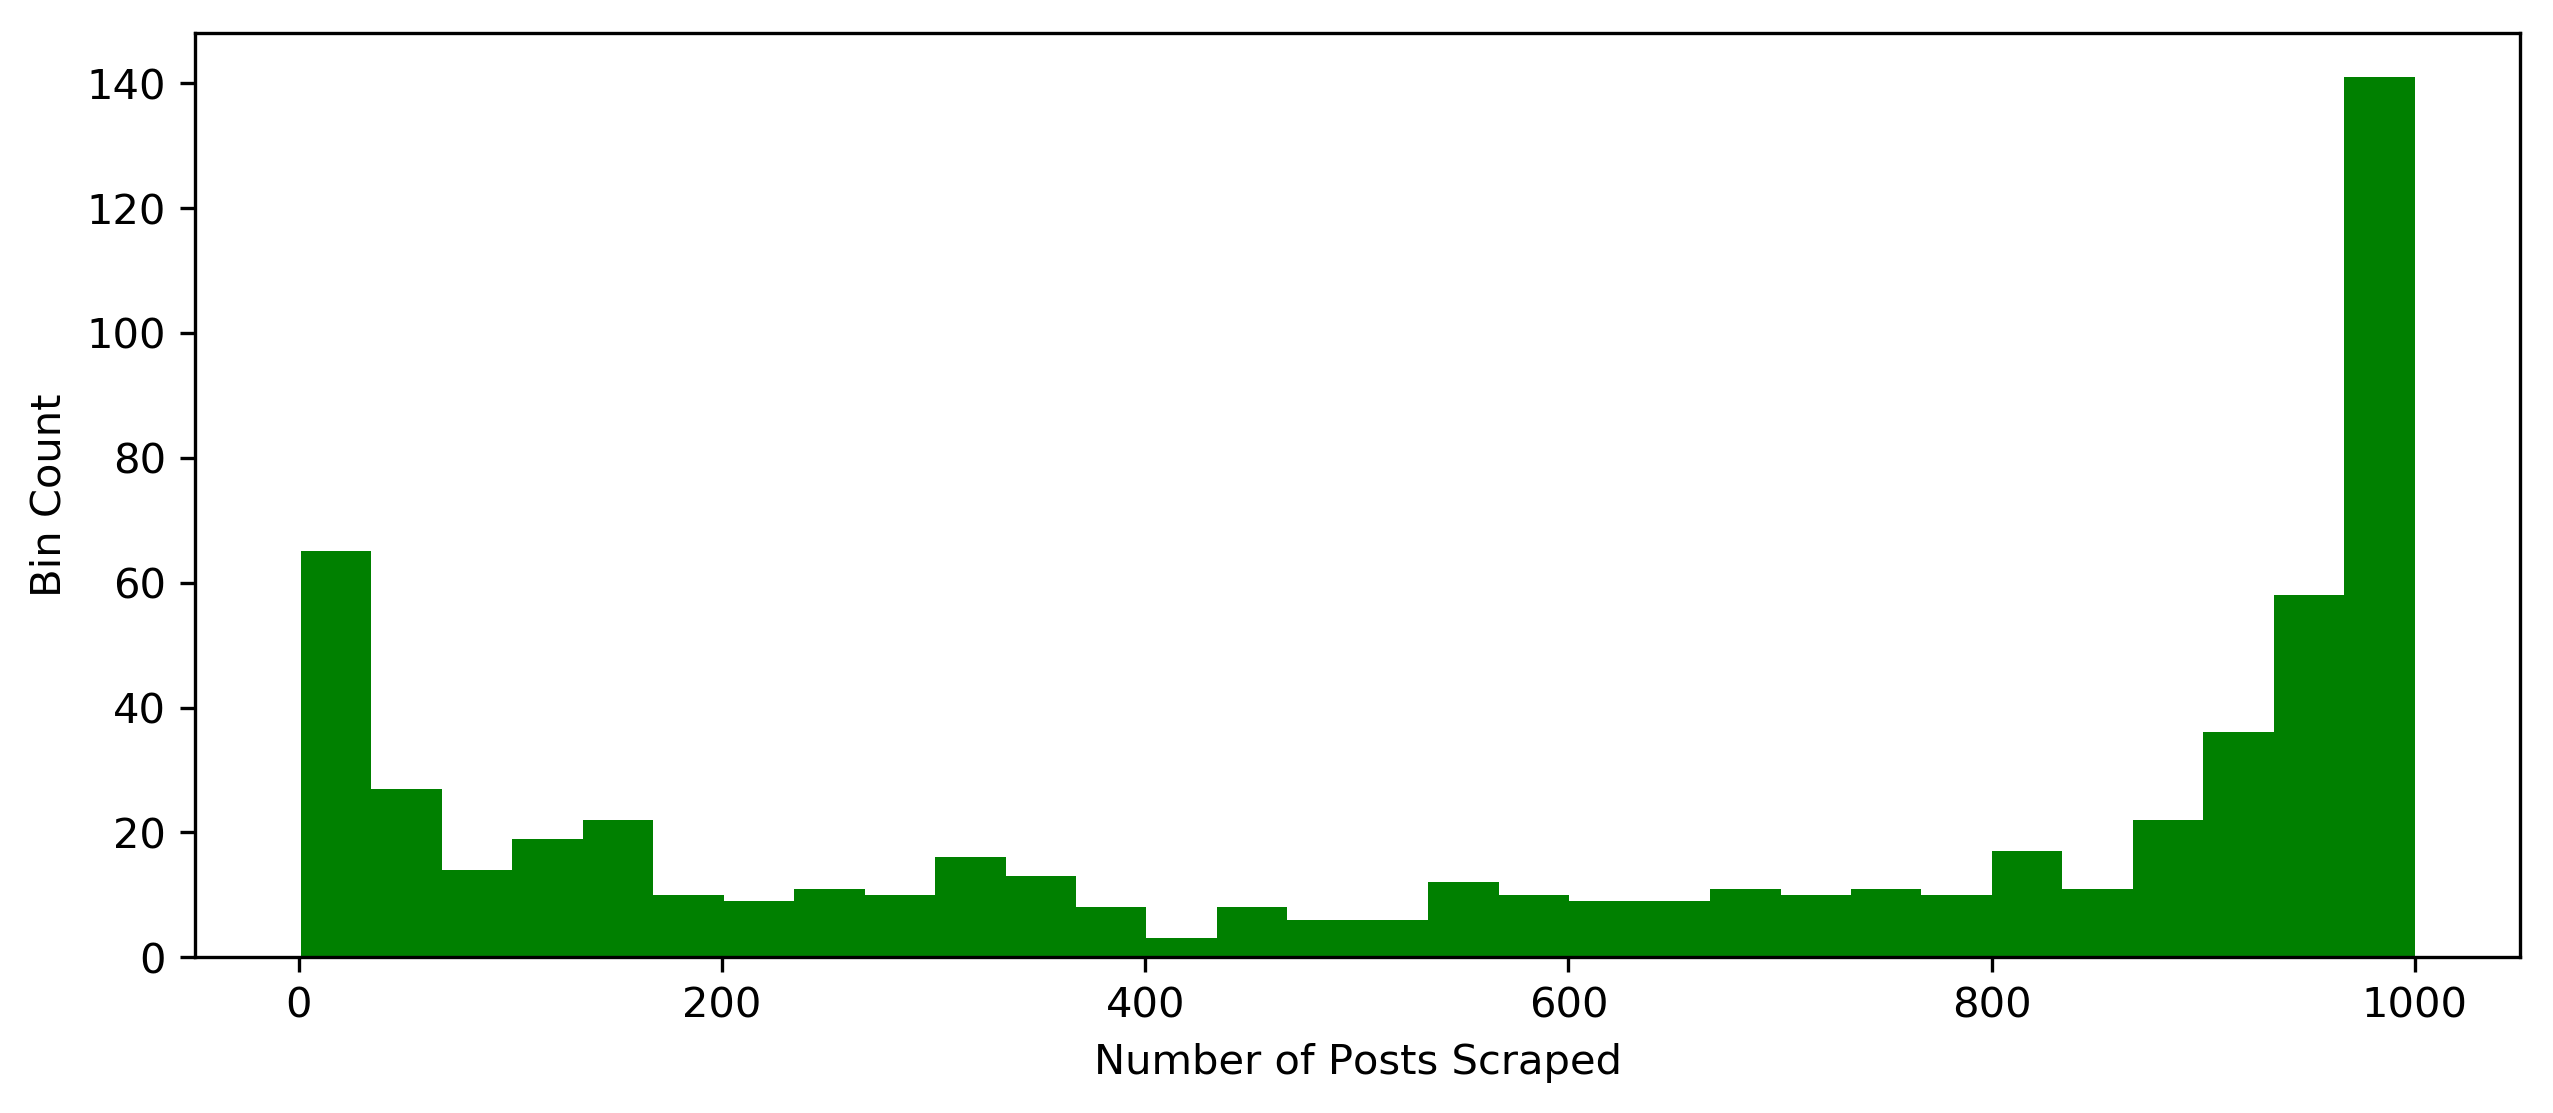
\includegraphics[width=\columnwidth]{images/Posts_Per_Page_Histogram.png}
    \caption{Histogram of the Number of Posts Scraped Per Facebook Page}
    \label{fig:histogram_posts_scraped}
\end{figure}


\subsubsection{Data Collection}
The researchers created a Python web scraper to crawl Facebook pages via the Facebook Graph API, a publicly available API. The top 1000 posts are scraped from each Facebook page, though most pages contain fewer than 100 posts. Figure-\ref{fig:histogram_posts_scraped} shows a histogram of the number of posts scraped from each Facebook page. In total, the study collected 366,415 Facebook posts and 1,305,375 million comments.  

\begin{figure}
\centering
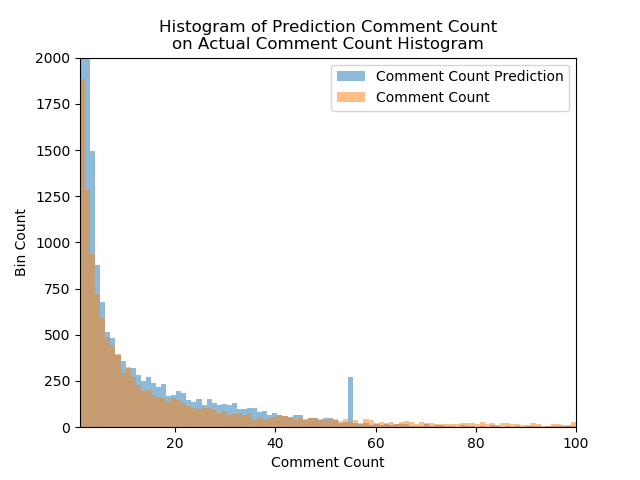
\includegraphics[width=\columnwidth]{images/Comment_Count_Prediction_vs_Actual.png}
\caption{Actual vs Predicted Comment Count Histogram}
\label{comment_count_histogram}
\end{figure}

\begin{figure}
\centering
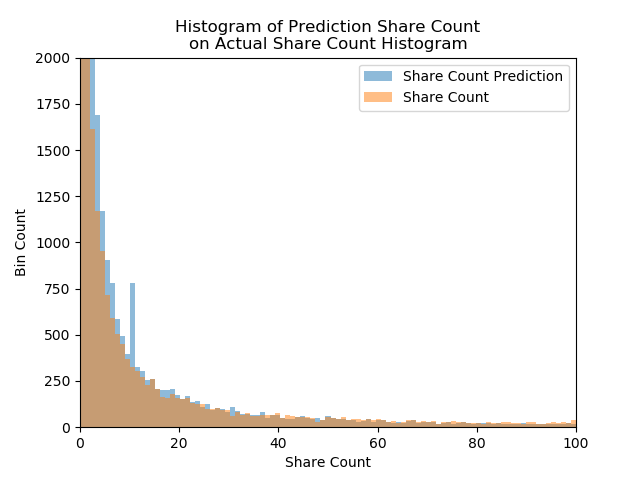
\includegraphics[width=\columnwidth]{images/Share_Count_Prediction_vs_Actual.png}
\caption{Actual vs Predicted Share Count Histogram}
\label{share_count_histogram}
\end{figure}

The study also analyzed comment sentiment scores for each post. This study made use of VADER, a parsimonious rule-based model for Sentiment Analysis of Social Media Text \cite{Gilbert} for its sentiment analysis. The sentiment analysis output was a score between -1 and 1, where 0 denotes neutral sentiment, -1 is very negative, and +1 a very positive sentiment. Posts with comments were given a sentiment score by averaging the sentiment score from all its comments.  Figure-\ref{comment_sentiment_histogram} shows a histogram of comment sentiments for the Facebook posts.

\begin{figure}
\centering
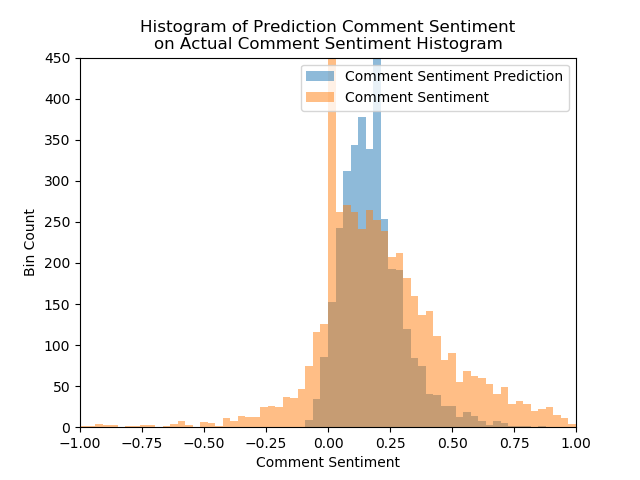
\includegraphics[width=\columnwidth]{images/Sentiment_Prediction_vs_Actual.png}
\caption{Actual vs Predicted Comment Sentiment Histogram}
\label{comment_sentiment_histogram}
\end{figure}

\subsubsection{Image Processing}
Images are inherently highly dimensional. In order to reduce the number of features created by using images as part of our machine learning algorithm, we took several steps to reduce each image’s dimensionality. First, we used principal component analysis. The number of dimensions to keep was set at 20 since the image variance is lower after denoising, reducing noise and data size. Image denoising can further reduce noise. Second, the research applied a Gaussian blur with a standard deviation of five to each image, which applies image blurring and emphasizes edges. Dilation and erosion are also applied to the image to remove noise in the edge space.

\subsection{Text Processing}
The method needs to transform text strings in order to create features for a neural network. Our process transformed text data into word vectors. First, the program split data into word tokens using whitespace as a delimiter. The program grouped these tokens into sentences, and both lowercased and removed common English stopwords and words with three or fewer characters. A port stemmer creates stems for all the words. A POS tag library performed parts-of-speech tagging. The program then extracted stems with a word lemmatizer, which takes the stem and the POS tag as input. Finally, the program fed the lemmatized text sentences to a td-IDF vectorizer. This created word vectors for training the neural network.

\subsection{Methodology}
The collected data consists of two types of data: text and image data. The text consists of Facebook posts and comments, and image data are any images attached to the post. These train and test this study's machine learning models. 

The machine learning models are separated into three groups, corresponding to the types of input data. The three types of input data were text-only data, image data, and input consisting of text and image data. Each input type had a corresponding machine learning architecture for training. For example, text data train a NN, images train on a CNN, and the combination of text and images train on a combined NN and CNN model. Thus, three input types for three types of models make a total of nine models.

\section{Results}
Our machine learning algorithm's output was training against each post's comment count, share count, and comment sentiment. The experiments use different sized data sets.  Comment and share count metrics utilized 366,415 posts in training and testing. Comment sentiment experiments included 201,215 posts. The comment sentiment data set was smaller due to limitations in the Facebook API.

The Python library Keras trained the machine learning models. The models predict continuous variables, which requires the model to perform regression. Keras provides many loss functions for regression.  The research's ultimate goal is to differentiate between ad performance, so the researchers chose a loss function that more heavily penalizes significant differences in user interaction, which is accomplished by choosing the Mean Squared Error (MSE) loss function since it has a squared loss penalty for any differences.  The combined model outperformed both the text-only and the image-only models for predicting all social media metrics.  Figure-\ref{mse_ratios} displays results as a ratio to the combined model's loss. 

\begin{table}[]
\centering
\begin{tabular}{lllll}
Metrics (MSE Ratio) & Text-Based NN & Image-Based CNN & Combined Decision Tree & Combined NN \\
Share Count       & 3.44 & 1.01 & 2.58 & 1.00 \\
Comment Count     & 1.02 & 1.01 & 1.29 & 1.00 \\
Comment Sentiment & 1.42 & 1.14 & 4.20 & 1.00
\end{tabular}
\caption{\label{tab:widgets}Model Mean Squared Error Reported as a Ratio to the Combined Neural Network Model's Mean Squared Error}
\end{table}

\subsubsection{Model Performance}
The combined model best predicted all user behavior metrics. Each machine learning model had its lowest MSE predicting for share count. The CNNs achieved a lower MSE than the NN on all metrics. Moreover, the CNN performance is best on data exhibiting a higher variance. Figure \ref{share_count_histogram} and \ref{comment_sentiment_histogram} show the predicted vs actual distribution for the combined model.

\subsection{Linear Models of Scraped Data}
This research created linear models to better understand the data before creating machine learning models. R scripts generated the linear models. The reported numbers are the coefficient of determination of the linear models. The linear models found an $R^2$ of 0.22 between talking about count and share count. The analysis found an $R^2$ of 0.38 between the fan count and talking about the count. The most significant result was an $R^2$ of 0.44 between comment sentiment and comment count. An $R^2$ of 0.38 and 0.44 are significant enough to create multicollinearity issues in machine learning features, which means that best practice avoids including two strongly correlated features. In addition, it is best practice to avoid correlated variables because they can negatively affect model weights by giving double the signal due to variable correlation. 

\subsection{Text-based NN Models}
This research utilized Keras to create, train, and test this model. Initial training experimented with 2-8 hidden layers. The final model utilized two hidden layers, as two layers performed similarly to eight hidden layers. This research initially experimented with word vector sizes from 1k-400k. Good performance and fast training occurred with a word vector size of 10k. The NN models used 10k as the word vector size.

\subsection{Image-based CNN Models}
Related work includes sections on keypoint descriptors and neural networks. CNNs detect image features and key points during repeated pooling and filter stages.  This replaces the usefulness of image descriptors. Applied research uses CNNs in favor of image descriptors. Moreover, CNNs were faster to train than comparing image descriptors between images. This research trained with as many as eight layers and as few as one hidden layer. Model depths above three trained to a similar degree of accuracy. The models experimented with different convolutional size sequences. The experiments include doubling in size, usually from 64 to 128, with a 2x2 filter. The alternative was reduced by size in half with a 2x2 filter.  Models with a 2x2 filter that decreased their size by half produced the highest accuracies. The final model contained four hidden layers. This research used this CNN configuration for all CNN model training. The final image-based model performed with a better loss than the text-based NN model on all metrics.   

\subsection{Combined Models}
The combined model concatenates both text-based NN and image-based CNN. The Keras API includes the ability to combine models. The API concatenated each model after the CNN flattened. At this point, the CNN portion has finished, and the remaining eight nodes form a NN. At the point of model concatenation, the NN also decreased to eight nodes. The result was a NN layer of sixteen densely connected nodes—the sixteen-node NN connected to a final output node.    
\subsection{Application}
The research applied the models in a real-world application. The application explored a use case to demonstrate the model's ability to choose which two advertisements would have the best performance. The research only compares advertisements with a significant value difference, where a significant difference is anything more than one standard deviation, as defined by the data distribution. The research found that models are unlikely able to differentiate between advertisements with similar performances. The combined model performs all predictions since it performed best across all metrics. Moreover, the application is the most useful if it can detect poor-performing and best-performing advertisements.  

The scenario is predicting user engagement for advertisements. The scenario pairs Facebook posts together. The model predicts user engagement for all posts. The program scores how often the model correctly predicted for greater user engagement. The program reports the result for each metric. The score is the number of correct predictions over incorrect predictions. This research compared the score with a random model. The random model produced the correct answer 50\% of the time. The combined model scored 93\% for comment sentiment, 65\% for comment count, and 63\% for share count.

The model performance shows its applicability in the real world.  Platforms could employ the models to aid advertisers in choosing the best performing advertisement before paying to advertise it on social media. The model can tell advertisers which ads would perform best on the platform, which allows advertisers have their ads vetted. The vetting could prevent advertisers from spending large amounts of money showing worse ads. Moreover, the vetting would allow advertisers to only show ads that will perform best. In the context of billions, 93\%, 65\%, and 63\% accuracy is a substantial monetary difference.

\subsection{Linear Models}
The data correlations were sensible. The metrics for comment count and share count are correlated. This correlation is sensible, considering that users talk about shared content. Moreover, the shared content is interesting. Shared content also creates more interesting content. Linear models also found a correlation between fan count and share count. The more fans a page has, the more opportunities exist for people to share the content. Alternatively, people are fans of the page because they like the content and if people like content, they are more likely to share it. 

Linear models also discovered a correlation between comment count and comment sentiment. Posts that receive many comments are likely to receive positive comments. We can infer that happier users comment at a higher rate, or positive content elicits more comments, which are also likely to be positive. Interestingly, comment count was not correlated to share count. One might infer that just because a post draws attention and comments does not mean they are likely to get shared. It might also mean that happier content, which receives more comments, does not cause users to share that content. Page metrics are also not correlated with comment count, i.e., a famous or less popular page did not necessarily generate more or fewer comments. The study uses the lack of correlation to justify comparing posts across Facebook pages.

\subsection{Metric Prediction}
The data correlations were sensible. The metrics for comment count and share count are correlated. This correlation is sensible, considering that users talk about shared content. Moreover, the shared content is interesting. Shared content also creates more interesting content. Linear models also found a correlation between fan count and share count. The more fans a page has, the more opportunities exist for people to share the content. Alternatively, people are fans of the page because they like the content and if people like content, they are more likely to share it. 

Linear models also discovered a correlation between comment count and comment sentiment. Posts that receive many comments are likely to receive positive comments. We can infer that happier users comment at a higher rate, or positive content elicits more comments, which are also likely to be positive. Interestingly, comment count was not correlated to share count. One might infer that just because a post draws attention and comments does not mean they are likely to get shared. It might also mean that happier content, which receives more comments, does not cause users to share that content. Page metrics are also not correlated with comment count, i.e., a famous or less popular page did not necessarily generate more or fewer comments. The study uses the lack of correlation to justify comparing posts across Facebook pages.
The machine learning models were quick to train. The large batch sizes of 256 helped initialize model weights and prevent overfitting. Employing the Adam optimizer also helped reduce training time. This research scaled the data using min-max scaling. Each type of model required a similar quantity of training time. 

Models with a higher variance achieved the worst overall loss/variance ratio.  It seems that the larger the data variance, the higher the resulting mode's MSE.  Share count had the highest variance of all the measured metrics, 1000x more than the comment count.  The high MSE likely reflects that share counts are less related to the image and text data. Share counts might be a factor of other features, like page popularity.

%Future work might include a third model with Facebook page metrics.

The combined model outperformed all other models for each metric. The result is even more surprising in light of the decision tree performance. The decision tree also took as input data from both the text-based NN and the image-based CNN. However, the decision tree performed far worse than the combined model. While the exact reason is unknown, there are a few differences between the two models. First, the combined model closely integrates with the text-based NN and image-based CNN. Second, when the combined model trains, it also trained its two-parent models. As a result, the decision tree did not learn alongside its inputs. Likely, parent models compensate for mistakes by training together.

The model concatenation occurs in the later stages of each model. The goal was to combine these dense networks before the final output and after the CNN. The goal was a combined model that kept parent model training more-so independent. Combining models at the end keeps both models somewhat separate. This research plotted prediction vs. test data for all models. The combined model best resembled the test data's distribution. The text-based NN and image-based CNN tended to skew towards zero due to spread predictions.

Image-based models performed better than text-based models on all metrics, likely because it emphasizes images' importance for predicting user interaction on social media. Text-based models were poor predictors for many metrics. Text-based models did especially badly in prediction share counts. One may guess that users are sharing content they consider worthy of sharing. 

%Later modeling compares the results against a random model. CNN with image inputs was more accurate than text-based NN.  This seems to say that images influence a large degree of the comment sentiment. 

\subsection{Model Loss and Outperforming Random Guessing}
In light of the newly created data, there are no other baseline measures for what constitutes good model performance. One goal was to produce a model that performed better than random guessing. Random guessing alone is not representative of the data. A better guess is based on the input's distribution. A good random guess would consider the data's value at each point along with its distribution. Such a distribution would weigh each value by the frequency of data. This calculation is the expected value. For a normal distribution, the expected value is equal to the mean. Also, each output in the research resembles the normal distribution after a log transformation. If the model always predicts the mean, the MSE is equal to the data's variance. The variance is a squared order of the data's distance from the mean. The MSE is also a squared order of the model's prediction from the actual value. Producing a model whose loss is below the variance is a general measure of demonstrating the model is doing a significant amount of learning. Fortunately, the combined model's performance was always much lower than each output data's variance.

\subsection{Study Contributions}
The study demonstrates the improved model performance by combining image and text data when predicting user behavior on social media.  The research found that machine learning with both image and text data results in enormous improvements for predicting comment sentiment.  This serves as a benchmark for predicting user sentiments on social media.  It also provides a comparison between text-based, image-based, and combined text and image model performance. The code is available on GitHub for future studies.

The research serves as a case study for combining text and image data. The study provides performant model hyperparameters in model depth, dropout rate, and word vector sizes.  The expected results will be generalizable to other studies and encourage others to explore understanding advertisement performance on social media.

\subsection{Addressing Research Questions}
This research question asks if a machine learning model, trained with text and image data, can predict user interaction on social media.  The research found that models utilizing image and text data outperformed their single-data type counterparts.  The research questions also asked how well the models can predict user interaction in terms of MSE and variance.  Each machine learning model achieved a MSE below the data variance, demonstrating a measure of model success learning user behavior. In addition, the combined model predicts which of two advertisements would evoke the more positive comment sentiment 93\% of the time, further confirming the model's successful performance.

\subsection{Limitations}
Model training time was a limitation. There were twelve models. Each model requires many hours of training time. Machines with GPUs can only train one model at a time, so this process was very time-consuming. Time was not sufficient to train all models thoroughly. With more time, the models could have reached lower losses.  One observation is that the models generally begin to overtrain after 30 epochs. More regularization might mitigate this problem. Such mitigations would likely lead to increased model performance. Heuristics dictated for hyperparameters and batch sizes. 

\subsection{Future Work}
Given that share count and comment sentiment have a coefficient of determination over 0.4, the share count model is likely a good input for predicting comment sentiment. Future research can incorporate this input to improve future models when predicting user behavior. In addition, future research could overcome existing Facebook API scraping problems. Another avenue for research is collecting comment sentiments for the 350k Facebook posts and using the new data to train better models.  Moreover, future work can incorporate the combined text and image model with the image-based CNN and text-based NN into an ensemble model to see if it improves performance.

The models created from this research could generate data to train a generative model.  The generative model could transform images and text into advertisements that should generate more user interaction.  The transformed and original advertisements could both be shown on social media and their user interactions compared. Thus, the study might demonstrate that generative models generate and improve existing advertising content.

\bibliographystyle{apacite}
\bibliography{references}   
 
\end{document}
